\section{Discussion}\label{discuss}
%VI.	Discussion
%	a.	\pacora in the Cloud
%	b.	Challenges
%		i.	Outliers/Performance Non-Monotonicity
%			1.	Possible Solutions
%				a.	Heuristics + Feedback
%				b.	Stochastic Models
%		ii.	Variability - can't just average
%			1.	Phases
%			2.	Input Dependent
%			3.	Other � such as network connection
%			4.	Shared Resources
%			5.	Possible Solutions
%				a.	Heuristics + Feedback
%				b.	Stochastic Models
%				c.	Changing Models

There are two main sources of challenges for \pacora's design: performance non-monotonicity and performance variability.  In the following section we describe possible techniques for coping with these challenges.

The main concern with performance non-monotonicity and variability is that they can possibly effect the accuracy of the response time functions.  However, an interesting result we have found while evaluating \pacora is that model accuracy has less impact on the quality of resource allocation decisions than anticipated.  When experimenting with possible models for the RTF functions, we found that while some models were always a little too inaccurate and did degrade the performance of the resource allocation decisions, once a model crossed a certain threshold of accuracy then better models provided insignificant improvement in resource allocation decisions~\cite{pacora_tr}. Figure~\ref{accuracy_quality} shows the effect of model accuracy on the quality of the resource allocation decisions made using RTF model in Equation~\ref{rtf_eq}.  Although there is a slight correlation between model accuracy and decision quality, many decisions with inaccurate models still result in near optimal allocations.
\begin{figure}[!t]
	\begin{center}	
%		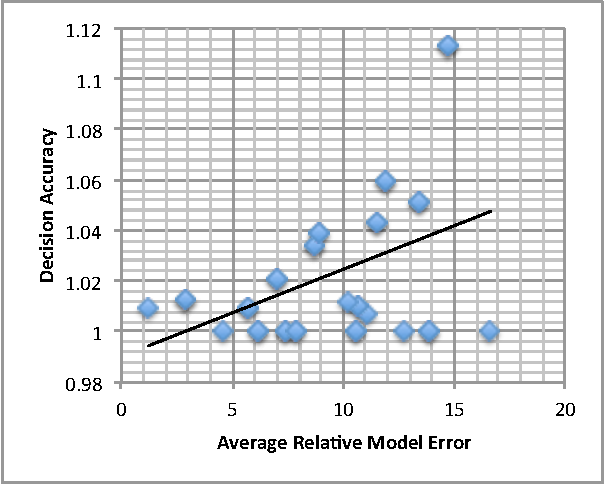
\includegraphics[width=0.9\textwidth]{cluster_decision_accuracy.pdf}
		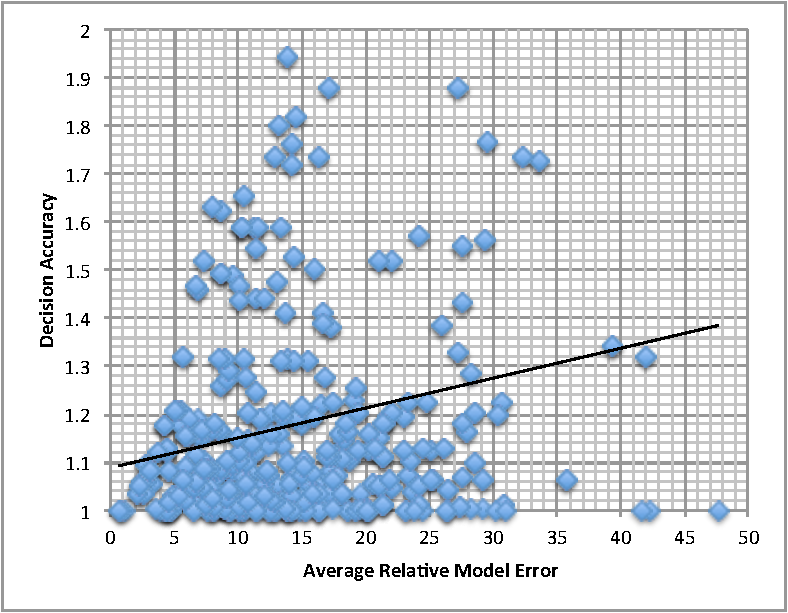
\includegraphics[bb=0 0 378 294,width=0.9\columnwidth]{parsec_decision_accuracy.pdf}
		\caption{Effect of Model Accuracy on Decision Quality}
		\label{accuracy_quality}
	\end{center}
\end{figure}

\subsection*{Outliers and Performance Non-Monotonicity}
Outliers and performance non-monotonicity can be handled with a combination of two techniques.  Outliers should be thrown out during the model creation phase as described in Section~\ref{model_creation} to prevent those points from distorting the accuracy of the other allocations.  In our study, we experienced outliers for a few applications with a particular number of hyperthreads and for many applications when given only one cache way.  The second part of the solution is keep track of these points with extreme error in the model and use heuristics to adjust the resource allocations to avoid such points.  We did not implement this second part in our current evaluation, but it is a subject of future study. 

Additionally as responsiveness, predictability, and efficiency increase in importance for systems, we expect to see an increased number of chip-designs that seek to provide more performance monotonicity thereby diminishing the issue of outliers.

\subsection*{Variability}

We observe three main sources of performance variability for applications: variability caused by phases in the application; applications whose performance changes as function of their inputs; and variability from resources such as interference from shared resources or non-deterministic resources such as network connection.

\subsubsection*{Phases}

As described in Section~\ref{model_creation}, phases can be handled with online creation of the RTFs.  However, another option is build different models per phase and to detect phase changes and swap models.  We used this method for the video application in Figure~\ref{video_experiment_wp} and ~\ref{video_experiment_battery}.  This approach has the advantage that it can more rapidly adapt to phases; however it requires identifying phases and additional space to store the extra models. Phase detection is an active area of research, and \cite{dhodapkar-micro03} provide an overview of techniques.  Another approach is to build a model that represents the resource requirements of the most demanding phase.  The system can be designed make use of the idle resources when available or power management mechanisms can put them in low-power mode.

\subsubsection*{Input Dependence}
Some applications may significantly change performance as a function of their inputs. In the case of our video application we ignored its input dependency without significant effect.  However for other applications the effect may be more pronounced.  One approach to handle may be to have multiple models for the application and based on the current input select one.  Another possible solution is to instead alter the RTFs to be stochastic models representing the response time of the application with a certain likelihood.  Stochastic models for \pacora are discussed in more detail in ~\cite{pacora_tr}.

\subsubsection*{Resource Variability}
In our study we experience resource variability both in the form of non-deterministic resources such as the network connection in {\tt tradebeans} and shared resources such as memory bandwidth. Stochastic models are most likely the right way to deal with non-deterministic resources and may be particularly necessary for representing hard drive-based storage in warehouse scale computing.

Shared resources can also be handled with stochastic models.  However since the models can be built online while other applications are running, in many cases the interference from a loaded machine is already captured in the model.  In our static allocation evaluation, we built the models in isolation but found that \pacora was still able to make near optimal resource allocations on average for a loaded machine despite the shared resources.

Obviously there may always be some shared resources; however, we have found a trend towards minimizing interference in emerging chip-designs as efficiency and predictability begin to trump utilization as primary concerns.


%other types of non-deterministic apps?



% don't forget cpu frequency






